
%%% main document {{{

\documentclass[
a4paper,     %% defines the paper size: a4paper (default), a5paper, letterpaper, ...
% landscape,   %% sets the orientation to landscape
% twoside,     %% changes to a two-page-layout (alternatively: oneside)
% twocolumn,   %% changes to a two-column-layout
 headsepline, %% add a horizontal line below the column title
% footsepline, %% add a horizontal line above the page footer
% titlepage,   %% only the titlepage (using titlepage-environment) appears on the first page (alternatively: notitlepage)
% parskip,     %% insert an empty line between two paragraphs (alternatively: halfparskip, ...)
% leqno,       %% equation numbers left (instead of right)
% fleqn,       %% equation left-justified (instead of centered)
% tablecaptionabove, %% captions of tables are above the tables (alternatively: tablecaptionbelow)
% draft,       %% produce only a draft version (mark lines that need manual edition and don't show graphics)
% 10pt         %% set default font size to 10 point
11pt         %% set default font size to 11 point
% 12pt         %% set default font size to 12 point
]{scrartcl}  %% article, see KOMA documentation (scrguide.dvi)



%%%%%%%%%%%%%%%%%%%%%%%%%%%%%%%%%%%%%%%%%%%%%%%%%%%%%%%%%%%%%%%%%%%%%%%%%%%%%%%%
%%%
%%% packages
%%%

%%%
%%% encoding and language set
%%%

%%% ngerman: language set to new-german
\usepackage{ngerman}

%%% babel: language set (can cause some conflicts with package ngerman)
%%%        use it only for multi-language documents or non-german ones
%\usepackage[ngerman]{babel}

%%% inputenc: coding of german special characters
\usepackage[utf8]{inputenc}

%%% fontenc, ae, aecompl: coding of characters in PDF documents
\usepackage[T1]{fontenc}
\usepackage{ae,aecompl}

%%%
%%% technical packages
%%%

%%% amsmath, amssymb, amstext: support for mathematics
%\usepackage{amsmath,amssymb,amstext}

%%% psfrag: replace PostScript fonts
\usepackage{psfrag}

%%% listings: include programming code
%\usepackage{listings}

%%% units: technical units
\usepackage{units}

%%% tiefgestellte zahlen
\usepackage{subscript}

%%% mathefoo
\usepackage{amsmath}


\usepackage{xcolor}
% TikZ-Bibliotheken
\usepackage{tikz}
 \usetikzlibrary{backgrounds}
 \usetikzlibrary{matrix}
 \usetikzlibrary{circuits.ee.IEC}
 \usetikzlibrary{positioning}
 
 
%Hintergrundstyle - optional
\tikzstyle{background rectangle}=
  [thick,draw=\lightgray, fill=white!99!black, rounded corners]
 
%Volt- und Amperemeter festlegen:
\tikzset{circuit declare symbol = ammeter}
\tikzset{set ammeter graphic ={draw,generic circle IEC, minimum size=5mm,info=center:A}}
\tikzset{circuit declare symbol = voltmeter}
\tikzset{set voltmeter graphic ={draw,generic circle IEC, minimum size=5mm,info=center:V}}
\tikzset{circuit declare symbol = generator}
\tikzset{set generator graphic ={draw,rectangle ee, minimum size=5mm,info=center:G}}
% Spannungs und Strompfeile
\tikzset{
  Pfeil/.style={thick,shorten >=#1,shorten <=#1,->}, % für Peile
  UPfeil/.style={blue,Pfeil=#1,font={\sffamily\itshape}},% für Spannungspfeile
  IPfeil/.style={red,Pfeil=#1,font={\ttfamily\itshape}} % für Strompfeile
}


%Boxen
\usepackage{empheq}
 
% Command "alignedbox{}{}" for a box within an align environment
% Source: http://www.latex-community.org/forum/viewtopic.php?f=46&t=8144
\newlength\dlf  % Define a new measure, dlf
\newcommand\alignedbox[2]{
% Argument #1 = before & if there were no box (lhs)
% Argument #2 = after & if there were no box (rhs)
&  % Alignment sign of the line
{
\settowidth\dlf{$\displaystyle #1$}  
    % The width of \dlf is the width of the lhs, with a displaystyle font
\addtolength\dlf{\fboxsep+\fboxrule}  
    % Add to it the distance to the box, and the width of the line of the box
\hspace{-\dlf}  
    % Move everything dlf units to the left, so that & #1 #2 is aligned under #1 & #2
\boxed{#1 #2}
    % Put a box around lhs and rhs
}
}

%%%
%%% layout
%%%

%%% scrpage2: KOMA heading and footer
%%% Note: if you don't use this package, please remove 
%%%       \pagestyle{scrheadings} and corresponding settings
%%%       below too.
\usepackage[automark]{scrpage2}


%%%
%%% PDF
%%%

\usepackage{ifpdf}

%%% Should be LAST usepackage-call!
%%% For docu on that, see reference on package ``hyperref''
\ifpdf%   (definitions for using pdflatex instead of latex)

  %%% graphicx: support for graphics
  %\usepackage[pdftex]{graphicx}

  \pdfcompresslevel=9

  %%% hyperref (hyperlinks in PDF): for more options or more detailed
  %%%          explanations, see the documentation of the hyperref-package
  \usepackage[%
    %%% general options
    pdftex=true,      %% sets up hyperref for use with the pdftex program
    %plainpages=false, %% set it to false, if pdflatex complains: ``destination with same identifier already exists''
    %
    %%% extension options
    backref,      %% adds a backlink text to the end of each item in the bibliography
    pagebackref=false, %% if true, creates backward references as a list of page numbers in the bibliography
    colorlinks=true,   %% turn on colored links (true is better for on-screen reading, false is better for printout versions)
    %
    %%% PDF-specific display options
    bookmarks=true,          %% if true, generate PDF bookmarks (requires two passes of pdflatex)
    bookmarksopen=false,     %% if true, show all PDF bookmarks expanded
    bookmarksnumbered=false, %% if true, add the section numbers to the bookmarks
    %pdfstartpage={1},        %% determines, on which page the PDF file is opened
    pdfpagemode=None         %% None, UseOutlines (=show bookmarks), UseThumbs (show thumbnails), FullScreen
  ]{hyperref}


  %%% provide all graphics (also) in this format, so you don't have
  %%% to add the file extensions to the \includegraphics-command
  %%% and/or you don't have to distinguish between generating
  %%% dvi/ps (through latex) and pdf (through pdflatex)
  \DeclareGraphicsExtensions{.pdf}

\else %else   (definitions for using latex instead of pdflatex)

  \usepackage[dvips]{graphicx}

  \DeclareGraphicsExtensions{.eps}

  \usepackage[%
    dvips,           %% sets up hyperref for use with the dvips driver
    colorlinks=false %% better for printout version; almost every hyperref-extension is eliminated by using dvips
  ]{hyperref}

\fi


%%% sets the PDF-Information options
%%% (see fields in Acrobat Reader: ``File -> Document properties -> Summary'')
%%% Note: this method is better than as options of the hyperref-package (options are expanded correctly)
\hypersetup{
  pdftitle={}, %%
  pdfauthor={}, %%
  pdfsubject={}, %%
  pdfcreator={Accomplished with LaTeX2e and pdfLaTeX with hyperref-package.}, %% 
  pdfproducer={}, %%
  pdfkeywords={} %%
}


%%%%%%%%%%%%%%%%%%%%%%%%%%%%%%%%%%%%%%%%%%%%%%%%%%%%%%%%%%%%%%%%%%%%%%%%%%%%%%%%
%%%
%%% user defined commands
%%%

%%% \mygraphics{}{}{}
%% usage:   \mygraphics{width}{filename_without_extension}{caption}
%% example: \mygraphics{0.7\textwidth}{rolling_grandma}{This is my grandmother on inlinescates}
%% requires: package graphicx
%% provides: including centered pictures/graphics with a boldfaced caption below
%% 
\newcommand{\mygraphics}[3]{
  \begin{center}
    \includegraphics[width=#1, keepaspectratio=true]{#2} \\
    \textbf{#3}
  \end{center}
}

%%%%%%%%%%%%%%%%%%%%%%%%%%%%%%%%%%%%%%%%%%%%%%%%%%%%%%%%%%%%%%%%%%%%%%%%%%%%%%%%
%%%
%%% define the titlepage
%%%

% \subject{}   %% subject which appears above titlehead
% \titlehead{} %% special heading for the titlepage

%%% title
\title{Messbericht \\ Diodenkennlinien}

%%% author(s)
\author{Felix Schiller \\ Sebastian Littau \\ E1FS2}

%%% date
\date{Reutlingen, am 08.03.2016}

% \publishers{}

% \thanks{} %% use it instead of footnotes (only on titlepage)

% \dedication{} %% generates a dedication-page after titlepage


%%% uncomment following lines, if you want to:
%%% reuse the maketitle-entries for hyperref-setup
%\newcommand\org@maketitle{}
%\let\org@maketitle\maketitle
%\def\maketitle{%
%  \hypersetup{
%    pdftitle={\@title},
%    pdfauthor={\@author}
%    pdfsubject={\@subject}
%  }%
%  \org@maketitle
%}


%%%%%%%%%%%%%%%%%%%%%%%%%%%%%%%%%%%%%%%%%%%%%%%%%%%%%%%%%%%%%%%%%%%%%%%%%%%%%%%%
%%%
%%% set heading and footer
%%%

%%% scrheadings default: 
%%%      footer - middle: page number
\pagestyle{scrheadings}

%%% user specific
%%% usage:
%%% \position[heading/footer for the titlepage]{heading/footer for the rest of the document}

%%% heading - left
\ihead[]{Schiller, Felix \\ Littau, Sebastian}

%%% heading - center
\chead[]{Messbericht \\Diodenkennlinien}

%%% heading - right
\ohead[]{\thepage}

%%% footer - left
% \ifoot[]{}

%%% footer - center
% \cfoot[]{}

%%% footer - right
% \ofoot[]{}



%%%%%%%%%%%%%%%%%%%%%%%%%%%%%%%%%%%%%%%%%%%%%%%%%%%%%%%%%%%%%%%%%%%%%%%%%%%%%%%%
%%%
%%% begin document
%%%

\begin{document}

% \pagenumbering{roman} %% small roman page numbers

%%% include the title
% \thispagestyle{empty}  %% no header/footer (only) on this page
\maketitle

%%% start a new page and display the table of contents
\newpage
\tableofcontents

%%% start a new page and display the list of figures
% \newpage
% \listoffigures

%%% start a new page and display the list of tables
% \newpage
% \listoftables

%%% display the main document on a new page 
% \newpage

% \pagenumbering{arabic} %% normal page numbers (include it, if roman was used above)

%%%%%%%%%%%%%%%%%%%%%%%%%%%%%%%%%%%%%%%%%%%%%%%%%%%%%%%%%%%%%%%%%%%%%%%%%%%%%%%%
%%%
%%% begin main document
%%% structure: \section \subsection \subsubsection \paragraph \subparagraph
%%%
\section*{Messaufgabe}
Zur Bestimmung der Eigenschaften einer Diode ist eine Messschaltung zur Aufnahme der Kennlinien $I=f(U)$ im Durchlassbereich unumgänglich. 

\section{Aufnahme der Kennlinie im Durchlassbereich}
\subsection{Messchaltung zur Aufnahme der Durchlasskennlinie}
\begin{center}
\begin{tikzpicture}[%show background rectangle,
circuit ee IEC, circuit symbol lines/.style={draw,thick},
font=\sffamily\upshape,
>=latex % Voreinstellung für Pfeilspitzen
]
\matrix (S) [
  matrix of nodes, nodes in empty cells,
  inner sep=0pt, outer sep=-.5\pgflinewidth,
  column sep=15mm, row sep = 7mm,
  nodes={minimum width=0pt}
  ]
{
  &&&  \\
  &&&  \\
  &&&  \\
  &&&  \\
  &&&  \\
  &&&  \\
};
 
 
%Orientierungshilfen
%\foreach \j in {1,...,6}
% \foreach \k in {1,...,4}{%
%\node[text=lightgray] at (S-\j-\k){+}; % Orientierungshilfe +
%\node[red, left] at (S-\j-1){\j}; %Orientierungshilfe Zeilennummer
%\node[red, above] at (S-1-\k){\k}; %Orientierungshilfe Spaltennummer  
%};%
 

%Bauteile
\draw (S-4-1) to  [generator={name=Gen}](S-2-1);

\draw (S-1-3) to  [resistor={info=R$_\mathsf{s}$, name=Wstd1}](S-3-3);
%\draw (S-4-3) to  [ammeter ={name=AM1}](S-6-3);
%\draw (S-1-4) to  [voltmeter ={name=VM1}](S-3-4);

\draw (S-4-3) to  [diode={info=D$_\mathsf{1}$, name=Diode}](S-6-3);
%\draw (S-4-5) to  [ammeter ={name=AM2}](S-6-5);
\draw (S-4-4) to  [voltmeter ={name=VM2}](S-6-4);

\draw (S-1-1) to  [ammeter ={name=AMg}](S-1-2);

%Spannungspfeile
%Spannungspfeil der Quelle / des Voltmeters
\draw[UPfeil=-1em]([xshift=-.5em]Gen.north west) -- node [left]{U$\mathsf{_G}$}([xshift=-.5em]Gen.south west);
%\draw[UPfeil=-1em]([xshift=.5em]VM1.north east) -- node [right]{U$\mathsf{_1}$}([xshift=.5em]VM1.south east);
\draw[UPfeil=-1em]([xshift=.5em]VM2.north east) -- node [right]{U$\mathsf{_{Diode}}$}([xshift=.5em]VM2.south east);
%\draw[UPfeil=-1em]([xshift=.5em]VM3.north east) -- node [right]{U$\mathsf{_3}$}([xshift=.5em]VM3.south east);
%\draw[UPfeil=-1em]([xshift=.5em]VM4.north east) -- node [right]{U$\mathsf{_4}$}([xshift=.5em]VM4.south east);

%Strompfeile
%\draw[IPfeil=-1em]([xshift=-.5em]AM1.north west) -- node [left]{I$\mathsf{_1}$}([xshift=-.5em]AM1.south west);
\draw[IPfeil=-1em]([yshift=.5em]AMg.north west) -- node [above]{I$\mathsf{_G}$}([yshift=.5em]AMg.north east);
 
%Leiterbahnen
\draw (S-1-1) -- (S-2-1);
\draw (S-1-2) -- (S-1-3);

%\draw (S-3-3) -- (S-3-4);
\draw (S-4-3) -- (S-4-4);
\draw (S-3-3) -- (S-4-3);


\draw (S-6-1) -- (S-6-4);
\draw (S-4-1) -- (S-6-1);
 
 
\end{tikzpicture}
\end{center}

\subsection{Aufbau der Schaltung}

Mithilfe der obigen Schaltung wird die Schleusenspannung für zwei gegebene Dioden bestimmt. Hierzu wird die entsprechende Diode mit einem in Reihe vorgeschalteten Schutzwiderstand versehen. Die Größe des Schutzwiderstandes wird berechnet, indem man mit der gegebenen maximalen Generatorspannung von 30V und der jeweiligen maximalen Strombelastung der Diode sowie eines angenommenen Schwellwertes von 1V bzw 2V unter Berücksichtigung der Gesetzmäßigkeiten der Reihenschaltung den benötigten Vorwiderstand berechnet. \newline
Für die Diode 1N4007 ergibt sich:
\[R_{S,Diode}=\frac{30V-0.93V}{100mA}=292\Omega \Rightarrow 270\Omega\]
Für die rote Leuchtdiode ergibt sich:
\[R_{S,LED}=\frac{30V-2V}{10mA}=2800\Omega \Rightarrow 2.7k\Omega\]
Es wird der nächstkleinere zur Verfügung stehende Widerstand ausgewählt. Damit wird erreicht, dass die angenommenen bzw. vorgegebenen Werte nicht zu weit überschritten werden.

\subsection{Messwerttabelle}

%\begin{center}
  \begin{tabular}{ l | c | c | c | c | c | c | c | c }
    \hline
    $U_{Diode}$ in V & 0    & 0.3    & 0.5    & 0.55    & 0.6   & 0.65    & 0.7    & 0.8   \\ \hline
    $I_G$ in mA      & 0    & 0      & 0.1    & 0.37    & 1.2   & 3.4     & 11.1   & 103   \\
    \hline
  \end{tabular}
  \newline
  \begin{tabular}{ l | c | c | c | c | c | c | c | c | c | c | c }
    \hline
    $U_{LED}$ in V & 1.3  & 1.4 & 1.5 & 1.6   & 1.65  & 1.7   & 1.75   & 1.8  & 1.9  & 2.0  & 2.075 \\ \hline
    $I_G$ in mA    & 0    & 0   & 0   & 0.002 & 0.006 & 0.025 & 0.085  & 0.2  & 2.44 & 6.44 & 10    \\
    \hline
  \end{tabular}
%\end{center}


\subsection{Belastungskennlinie}
Die gemessenen Werte lassen sich in einem Diagramm darstellen.

\begin{figure}[hbtp]
\centering
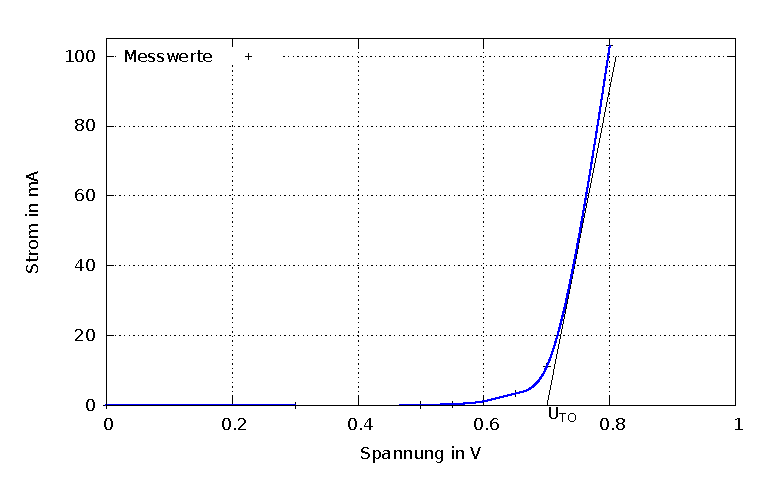
\includegraphics[scale=1]{kennlinie_diode.eps}
\caption{Kennlinie der Diode 1N4007}
\end{figure}

\begin{figure}[hbtp]
\centering
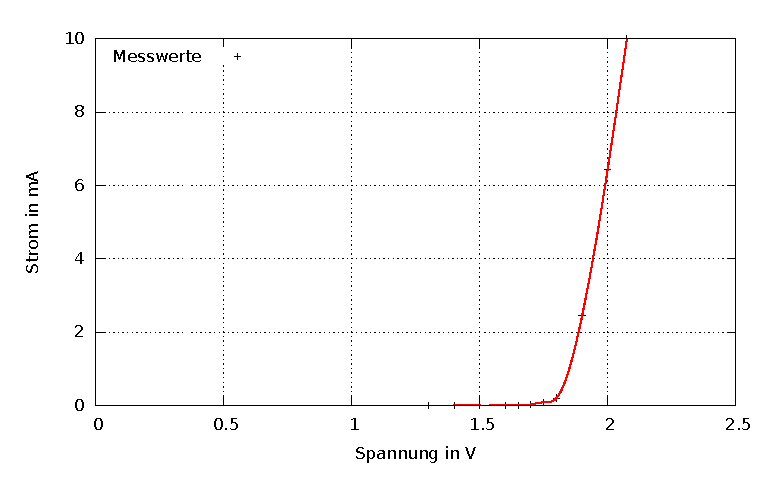
\includegraphics[scale=1]{kennlinie_led.eps}
\caption{Kennlinie der roten LED}
\end{figure}
\newpage

\subsection{Ermittlung der Schleusenspannung $U_{TO}$}

Die Schleusenspannung wird grafisch ermittelt, indem eine Gerade tangential an den Punkt der Belastungskennlinie angelegt wird, in welchem Sie die größte Steigung hat. Der Schnittpunkt mit der x-Achse ergibt dann die Schleusenspannung.
Durch dieses Verfahren ergibt sich für die Diode 1N4007 eine Schleusenspannung von ca. 0.7V, bei der roten LED eine Schleusenspannung von ca. 1.85V

\subsection{Vorwiderstand für drittes Bremslicht eines PKWs}

Gegeben sind 6 identische LEDs mit jeweils einem Strombedarf von $I_F = 15mA$ und einer Schleusenspannung von $U_{TO} = 2V$.
Die anliegende Versorgungsspannung ist mit $U_G = 13.4V$ angegeben.
Wir entscheiden uns dazu, die Dioden in Reihe zu schalten, demnach ergibt sich aufgrund der Gegebenheiten einer Reihenschaltung ein Gesamtspannungsabfall von $U_{Diodenreihe} = 6 \cdot 2V = 12V$. Somit muss ein Vorwiderstand gewählt werden, an dem exakt 1,4 Volt abfallen. Die 15mA die jede Diode benötigt bedeuten, dass auch am Widerstand 15mA anliegen, da in einer Reihenschaltung überall die gleiche Menge an Strom fließt. Somit ergibt sich für den Vorwiderstand:
\[R_{S,Diode}=\frac{1,4V}{0,015A}=93,3333\Omega\]
Es muss ein Vorwiderstand mit $93,3333\Omega$ gewählt werden.

\subsection{Verlustleistung am Vorwiderstand}

Die Verlustleistung am Vorwiderstand wird mithilfe der allgemeinen Formel für die Leistung berechnet.
Es gilt \[P = U\cdotI\]
In unserem Fall also \[P = 1.4V \cdot 15 mA = 21 mW\]
Die Verlustleistung an unserem Vorwiderstand beträgt $21 mW$.

%%%
%%% end main document
%%%
%%%%%%%%%%%%%%%%%%%%%%%%%%%%%%%%%%%%%%%%%%%%%%%%%%%%%%%%%%%%%%%%%%%%%%%%%%%%%%%%

% \appendix  %% include it, if something (bibliography, index, ...) follows below

%%%%%%%%%%%%%%%%%%%%%%%%%%%%%%%%%%%%%%%%%%%%%%%%%%%%%%%%%%%%%%%%%%%%%%%%%%%%%%%%
%%%
%%% bibliography
%%%
%%% available styles: abbrv, acm, alpha, apalike, ieeetr, plain, siam, unsrt
%%%
% \bibliographystyle{plain}

%%% name of the bibliography file without .bib
%%% e.g.: literatur.bib -> \bibliography{literatur}
% \bibliography{FIXXME}

\end{document}
%%% }}}
%%% END OF FILE
%%%%%%%%%%%%%%%%%%%%%%%%%%%%%%%%%%%%%%%%%%%%%%%%%%%%%%%%%%%%%%%%%%%%%%%%%%%%%%%%
%%% Notice!
%%% This file uses the outline-mode of emacs and the foldmethod of Vim.
%%% Press 'zi' to unfold the file in Vim.
%%% See ':help folding' for more information.
%%%%%%%%%%%%%%%%%%%%%%%%%%%%%%%%%%%%%%%%%%%%%%%%%%%%%%%%%%%%%%%%%%%%%%%%%%%%%%%%
%% Local Variables:
%% mode: outline-minor
%% OPToutline-regexp: "%% .*"
%% OPTeval: (hide-body)
%% emerge-set-combine-versions-template: "%a\n%b\n"
%% End:
%% vim:foldmethod=marker
